\chapter{Fundamentos teóricos}\label{chap:fundamentos}

\section{Enfermedad de Parkinson}

\subsection{Epidemiología y Etiología}
La \gls{enfermedad_de_Parkinson} (EP) es un trastorno neurodegenerativo multisistémico y de presentación generalmente esporádica, que afecta al sistema nervioso central provocando la aparición de síntomas motores y no motores \cite{E2004}. Es una enfermedad crónica -es decir, que persiste durante un extenso período de tiempo- y progresiva, lo que significa que sus síntomas empeoran con el tiempo. Su etiología desconocida conlleva a una patología aun mas compleja \cite{3249850720080101}; sin embargo, se cree que está relacionada con la acción e interacción de diversos factores genéticos y ambientales, que actúan como factores de susceptibilidad o precipitantes \cite{CAMPDELACREU2014541}.

Fue descrita por primera vez por James Parkinson en el año 1817 \cite{JamesParkinson2002}, siendo actualmente la segunda enfermedad neurodegenerativa más frecuente después de la enfermedad de Alzheimer, y se estima una predominancia luego de los 60 años \cite{GOMEZGONZALEZ2019396,CHAVEZ-LEON2013}. Es fundamental evaluar y cuantificar el impacto de la enfermedad en la población, particularmente en Uruguay. De esta manera, se pudo constatar que:

\begin{itemize}
    \item Alrededor del 3\% de la población mundial mayor a los 65 años padece la enfermedad de Parkinson \cite{Patel2009}, pudiendo alcanzar una prevalencia del 4\% en pacientes mayores de 80 años \cite{DeLauBreteler}
    \item En el año 2005, en las cinco naciones de Europa occidental y las diez más pobladas del mundo, representando 2/3 de la población mundial, el número de personas mayores de 50 años con EP estaba entre 4.1 y 4.6 millones. Se espera que este número ascienda entre 8.7  y 9.3 millones de parkinsonianos para 2030 \cite{Dorsey2007ProjectedNO}
    \item A principio del año 2018, un estudio de prevalencia de la EP en Norte América para las personas con edad mayor o igual a los 45 años, estimó que la prevalencia de la enfermedad era de 572 por 100.000 (intervalo de confianza del 95\%). Es decir, que habían unos 680.000 individuos en los EE. UU. con EP para el año 2010, que ese número aumentaría a unos 930.000 aproximadamente en 2020 y 1.238.000 para el año 2030 según las proyecciones de la población de la Oficina del Censo de los EE. UU \cite{Marras2018}
\end{itemize}

En cambio, no se encontró evidencia científica respecto a la prevalencia de la EP en Uruguay con datos actualizados y fiables. En el año 1993, se realizó un estudio de prevalencia de las enfermedades Neurodegenerativas donde se concluye que la prevalencia de la EP era de 1.36 casos cada 1000 habitantes \cite{AljanatiR2012}. Sin embargo, el estudio resulta arbitrario debido a la metodología utilizada, donde  en una primera fase consistió en una encuesta puerta a puerta -acotada a la ciudad de Migues, Canelones-; adecuada para la época pero obsoleta en la actualidad. Además, como se pudo ver en los estudios de prevalencia en otras regiones, la población afectada por la EP varía año a año. 

%Mas cifras
Por otro lado, el estudio reportado en \cite{Dorsey2018}, estima la carga global de la enfermedad de Parkinson entre 1990-2016, y busca identificar tendencias asociadas al trastorno (GBL, del ingles Global Burden of Disease). Según los resultados alcanzados, en 2016, 6.1 millones de individuos en todo el mundo padecían la EP, de los cuales 2.9 millones (47.5\%) eran mujeres y 3.2 millones (52.5\%) eran hombres afectados. Un total de 2.1 millones (34.4\%) de estos individuos provenían de países con un índice socio-demográfico (SDI) alto, 3.1 millones (50.8\%) de países con SDI medio o medio alto, y un 0.9 millones (14.8\%) de países con SDI medio o bajo. 

\noindent A nivel mundial, la enfermedad de Parkinson causó 211.296 muertes -93.512 mujeres y 117.784 hombres- y 3.2 millones de años perdidos debido a enfermedad, discapacidad o muerte prematura (AVAD, años de vida ajustados por discapacidad) -1.4 millones en mujeres; 1.8 millones en hombres- en 2016. Se entiende por AVADs como la suma de los años de vida perdidos (YLL, siglas en ingles, Years of Life Lost) y los años vividos con la discapacidad (YLD, siglas en ingles, Years Lost due to Disability). La figura Fig. \ref{fig:yll_yld} permite visualizar las tasas de YLL y YLD según la edad; así, el aumento relacionado con la edad fue considerablemente más pronunciado para los YLL que para los YLD, lo que sugiere que la letalidad para la EP aumenta con la edad.

\begin{figure}[H]
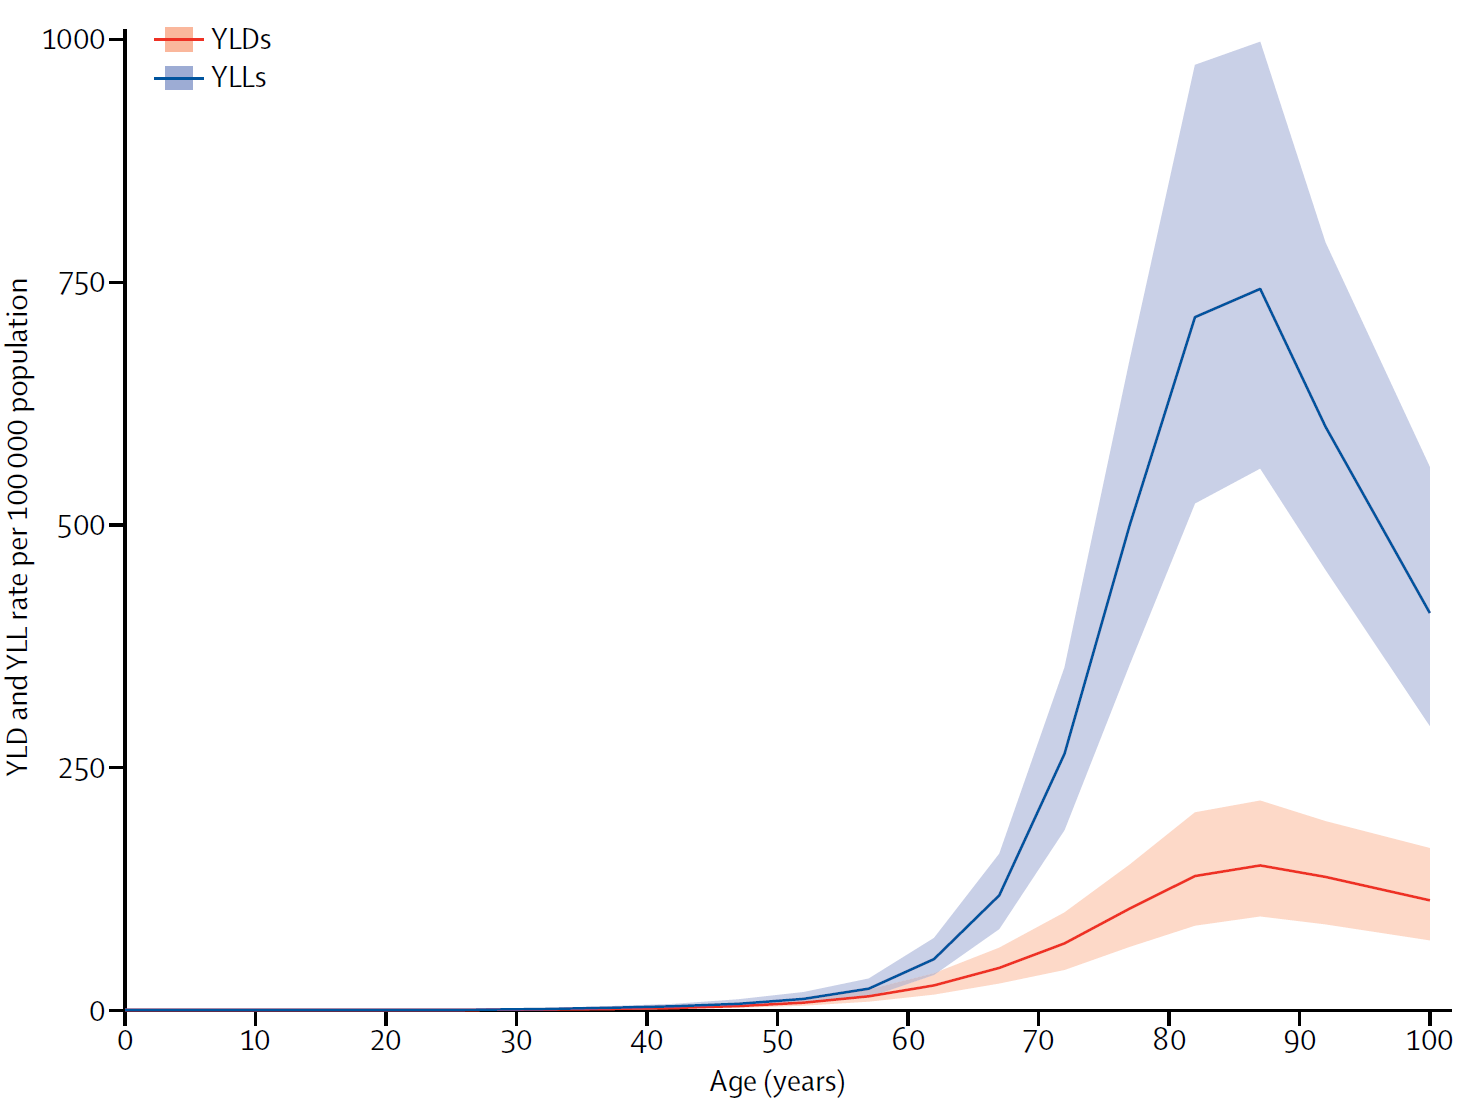
\includegraphics[width=\textwidth]{TESIS/imagenes/chap02/yll_yld.PNG}
\caption{ Tasas de años vividos con la discapacidad (YLD) y años de vida perdidos (YLL) cada 100.000 habitantes debido a la Enfermedad de Parkinson por edad, 2016. El sombreado indica intervalos de confianza del 95\%. \cite{Dorsey2018} }
\label{fig:yll_yld}
\end{figure}

\noindent En resumen, algunos hallazgos logrados fueron que:

\begin{itemize}
    \item El número de individuos con la EP en 2016 fue 2.4 veces mayor que a la de  1990. Dicho aumento no se explicó exclusivamente por un número cada vez mayor de personas adultas, ya que las tasas de prevalencia estandarizadas por edad aumentaron en un 21.7\% desde 1990 a 2016 en comparación con un aumento del 74.3\%  para las tasas brutas
    \item El número de muertes fue 2.6 veces mayor y el número de AVADs fue 2.5 veces mayor en 2016 que en 1990. Similar a la prevalencia, los aumentos no se explican solo por un número creciente de personas mayores, ya que las tasas estandarizadas por edad aumentaron en un 20\% tanto para las muertes como los AVADs
    \item La EP era poco frecuente antes de los 50 años de edad. La prevalencia en 2016 aumentó con la edad a partir de entonces y alcanzó un máximo entre los 85 y los 89 años (1.7\% para hombres; 1.2\% para mujeres) y disminuyó después de esa edad
\end{itemize}

\noindent La tabla Tab. \ref{ep_paises} ilustra los indicadores de defunciones, de prevalencias y las tasas AVADs a nivel mundial y en América del sur, especialmente Uruguay.

\begin{table}[H]
\begin{center}
\caption{Defunciones, prevalencia y AVADs (años de vida ajustados por discapacidad) para la enfermedad de Parkinson en 2016, y cambio porcentual entre 1990 y 2016 en las tasas estandarizadas por edad y por ubicación. \cite{Dorsey2018}} \label{ep_paises}
\hspace*{-2cm}%
\begin{tabular}{|p{2cm}|p{2cm}|p{2cm}|p{2cm}|p{2cm}|p{2cm}|p{2cm}|}
\hline
 & \multicolumn{2}{c|}{Decesos} & \multicolumn{2}{c|}{Prevalencia} & \multicolumn{2}{c|}{AVADs} \\
\hline
& En 100.000 (2016) & Tasa de cambio (1990–2016) & En 100.000 (2016) & Tasa de cambio (1990–2016) & Cantidad (2016) & Tasa de cambio (1990–2016) \\
\hline
Global & 2,83 & +19,5\% & 81,2 & +21,7\% & 3.234.514 & +22,1\% \\
\hline
América del sur & 0,98  & +3,1\% & 28 &  +5,4\% & 57.932 & +4,3\% \\
\hline
Uruguay & 8,38 & +7,1\% & 183,6 & +10,9\% & 3.775 & +8,2\% \\ \hline
\end{tabular}
\end{center}
\end{table}

\subsection{Sintomatología de la patología}

La alteración de la marcha es el síntoma primario del trastorno \cite{Jankovic}, y junto con las caídas causa pérdida de independencia en los sujetos afectados \cite{Ashburn}. Se caracteriza por deficiencias motoras, que incluyen esencialmente \cite{Rogers,Stamatakis,Hausdorff,Lord}: 
\begin{itemize}
    \item Temblor en las extremidades
    \item Aumento de la rigidez de las mismas
    \item Alteraciones de los parámetros espacio-temporales y fases de la marcha (p. ej. disminución de la longitud del paso y la velocidad de la marcha, variabilidad de zancada a zancada, fases de marcha)
    \item Ralentización del movimiento, marcha arrastrada o un inicio de marcha retrasado 
\end{itemize}

Otro evento frecuente, es la congelación de la marcha (FOG, del ingles, Freezing of gait), dado por una interrupción paroxística de la zancada o una marcada reducción en el avance hacia adelante del pie, que afecta gravemente la calidad de vida, aumenta el riesgo de caídas y fracturas en los sujetos afectados \cite{Perez-Lloret2014,Bloem2004}. En pacientes con EP, la investigación fisiopatológica de la FOG es bastante desafiante ya que se encuentra influenciada de manera crucial por una serie de factores cognitivos, atencionales, emocionales e incluso ecológicos \cite{Professor2008,Barthel2016}.

La cualidad progresiva de la enfermedad, conlleva a que las características motoras se vuelven cada vez más incapacitantes y las características no motoras menos tratables (p. ej. la demencia), acentuando la problemática de la enfermedad. Asimismo, los trastornos de la inestabilidad postural y las alteraciones de la marcha, no se traducen únicamente en alteraciones de aspectos cinemáticos como los mencionados; sino también en aspectos relacionados con su variabilidad, manifestaciones clínicas que de forma progresiva causan limitaciones en las funciones del paciente que impactan directamente en su calidad de vida y restringiendo tanto su actividad como su participación social \cite{DILLMANN2014882,MUNOZHELLIN2013190,FernandezDelOlmo2004,GOMEZGONZALEZ2019396}.

\subsection{Rehabilitación convencional}

En la actualidad, todas las terapias existentes para el manejo de los síntomas basadas en el uso de medicamentos dopaminérgicos, como la L-Dopa (levodopa) y agonistas de los receptores de \gls{dopamina}, han demostrado una pérdida de eficacia a lo largo del tiempo. A su vez, se han asociado con una variedad de efectos secundarios que incluyen \gls{discinesias} y fluctuaciones motoras, que pueden incluso empeoran las deficiencias motoras propias de la enfermedad.

Con el fin de lograr una evaluación cuantitativa más objetiva de la gravedad de los síntomas de la EP, determinar con mayor precisión el grado de progreso de la enfermedad, ajustar la medicación en la atención clínica de rutina o para su uso como medidas de resultados en ensayos clínicos, los neurólogos se apoyan en las escalas de evaluación semi cuantitativa, como lo es la Escala Unificada de Clasificación de la Enfermedad de Parkinson -elaborada por la Sociedad de Trastornos del Movimiento- (MDS-UPDRS, por sus siglas en ingles) \cite{Jellinger2002}. La escala MDS-UPDRS consiste en diversas partes, que buscan evaluar los síntomas motores y no motores a través de encuestas respondidas por el paciente, y evaluaciones basadas en exámenes realizadas por un médico capacitado. La principal limitación de esta evaluación es ser intrínsecamente subjetiva, con una significativa variabilidad entre los evaluadores en las puntuaciones \cite{Parisi2015}. Además, es una tarea que requiere mucho tiempo -difícil de lograr en sesiones clínicas-, y a la vez la presencia física de los pacientes en un entorno clínico donde se pueda obtener la evaluación. El Apéndice \nameref{appendix:MDS-UPDRS} permite visualizar la evaluación clínica mediante la escala MDS-UPDRS.

\subsubsection{Fisioterapia y rehabilitación}

A medida que la enfermedad progresa, la mayoría de las alteraciones del equilibrio y la marcha se vuelven resistentes a los tratamientos farmacológicos y quirúrgicos \cite{Rubinstein2002}. En consecuencia, para sortear el déficit de dopamina, la fisioterapia y la rehabilitación (i.e. estiramiento, fortalecimiento muscular, movimientos de las extremidades con pelotas y materiales de juego, acondicionamiento en bicicleta) pueden ser efectivas para contrarrestar las deficiencias motoras \cite{Fox2008}. 

La finalidad de la terapia de rehabilitación, es mejorar o mantener la calidad de vida de los sujetos afectados conforme a aumentar la movilidad, mejorar el equilibrio, la coordinación, reeducar la marcha para lograr la autonomía del paciente. Si bien ésta terapia no detiene la progresión de la enfermedad, habilita a prolongar la funcionalidad y reducir la incapacidad motora perfeccionando la marcha, las destrezas propioceptivas y desarrollando estrategias para conservar la independencia en las \gls{actividades_de_la_vida_diaria} elementales.

De esta manera, la rehabilitación debe atender al paciente según sus necesidades, su discapacidad, el estadio evolutivo de la enfermedad y las expectativas del paciente -similar a todas las enfermedades crónicas y progresivas-. 
A modo de ejemplo, se describen las fases y actividades del tratamiento de acuerdo a su evolución y al protocolo clínico a seguir \cite{MINISTERIO2010}:

\begin{enumerate}
    \item Fase Inicial
    \begin{itemize}
        \item Prevenir y tratar la inestabilidad postural.
        \item Evaluar e identificar tempranamente los problemas relacionados con alteraciones del movimiento.
        \item Fomentar la participación del paciente con EP en programas diseñados para mejorar la condición física general. (Cardiovascular, músculo esquelética, y neuromuscular).
        \item Prevenir las deficiencias posturales, deficiencias en marcha y traslado.
        \item Tratar la debilidad muscular y/o la rigidez articular.
        \item Utilizar estrategias de movimientos a lo largo de la enfermedad.
        \item Informar y Educar en salud, acerca de la enfermedad a los pacientes, familiares y cuidadores.
    \end{itemize}   

    \item Fase de Mantenimiento
    \begin{itemize}
        \item Tratar el deterioro músculo esquelético.
        \item Reeducar marcha y traslados. Prevención de caídas.
        \item Evaluar el medio en donde se desenvuelve el paciente (entrenamiento en el hogar y comunidad).
        \item Aplicar estrategias funcionales.
        \item Evaluar la prescripción de AT e instruir en su uso adecuado.
    \end{itemize}

    \item Fase Avanzada o tardía
    \begin{itemize}
        \item Asegurar el manejo adecuado de movimiento y posición.
        \item Evitar las caídas.
        \item Prevenir lesiones trofocirculatorias y posturales.
        \item Prevenir y tratar los problemas respiratorios.
    \end{itemize}
\end{enumerate}

Otra metodología muy empleada en la fisioterapia y rehabilitación, es la aplicación de incentivos o guías externas del tipo auditivo (i.e. a modo de metrónomos o golpes rítmicos en el suelo) o visual (i.e. huellas o líneas perpendiculares marcadas en el suelo) para mejorar los trastornos de la marcha; es decir, \gls{reeducar_la_marcha}. Si bien la evidencia científica existente respecto a la reeducación de la marcha es reducida, muchas investigaciones han concluido y reportado los siguientes resultados:

\begin{itemize}
    \item Viabilidad de generación de patrones adecuados de la marcha. Según \cite{MorrisME1994,Morris1996}, es posible que los parkinsonianos en presencia de estimulación sensorial regular, generen patrones adecuados de la marcha, corroborando una mejoría en los parámetros espacio-temporales bajo el uso de estímulos externos.
    
    \item Factibilidad de incidencia sobre el \gls{SNC}. Con fundamento en el principio de que todo acto motor es una elaboración del SNC -en respuesta a múltiple información sensitivo motora, simultánea y secuencial-, en efecto, se concluye que el segundo puede verse afectado o modificado positivamente mediante diversos estímulos táctiles, propioceptivos, auditivos, visuales, entre otros \cite{Moros2000}.
    
    \item Capacidad adaptativa del encéfalo. Existe evidencia científica que comprueban las propiedades de flexibilidad y modificabilidad del cerebro en distintos contextos -durante la infancia y la adolescencia, durante la edad adulta, como también en situaciones de lesión cerebral-. Así, el encéfalo puede alterase para adaptarse a diversas circunstancias \cite{Garces2014}.
    \item Estimulación visual sobre la marcha. El Neurólogo Británico James Purdon Martin,  logró demostrar el efecto positivo de las señales visuales sobre la marcha en la EP en el año 1967. Comprobó cómo tan solo una serie de líneas de color dispuestas en el suelo -de forma perpendicular a la dirección del movimiento-, mejoraban las características de la marcha de estos pacientes  \cite{Ostrosky2000,PALACIOSNAVARRO201649,Mille2012, ilianaloyola2017}.
    \item Resultados alentadores. Sidaway -entrenamiento con señales visuales- \cite{Moros2000}, logro una mejoría duradera en la velocidad de la marcha y en la longitud del paso incrementando la estabilidad del control motor subyacente responsable de la marcha. La investigación de \cite{Dias2017TREINODM} -señales visuales y terapia convencional-, aumentó la velocidad,la longitud de zancada y la cadencia al caminar, mejoró el equilibrio y la independencia en las actividades funcionales. Las sesiones experimentales en \cite{Almeida2012}, lograron mejoras  significativas de la longitud del paso, mejorando así la velocidad de la marcha -un incremento aproximado de 10 cm/s).
\end{itemize}

Conforme a lo mencionado, lograr una evaluación clínica con resultados confiables puede ser muy complejo y poco práctico, ya que requiere una supervisión continua de los sujetos afectados por parte del personal médico, o auto-informes realizados por los mismos pacientes (lo que probablemente sea subjetivo). El aumento de las disfunciones motoras a medida que avanza la enfermedad requiere evaluar cuantitativamente y controlar las alteraciones de la marcha con el tiempo. Asimismo, los neurólogos solo pueden confiar en observaciones cualitativas en sesiones esporádicas y basadas en su experiencia. De este modo, contar con una evaluación clínica precisa de la gravedad de estos síntomas y un seguimiento continuo (p. ej. un instrumento que actuara directamente sobre el desempeño de la marcha sería de utilidad mayor), es fundamental para identificar una terapia efectiva.

 
\subsection{Nuevo paradigma de Rehabilitación}

Con fundamento en las limitaciones clínicas mencionadas en el tratamiento convencional del trastorno para identificar, evaluar y monitorear la enfermedad de parkinson, la Ingeniería Biomédica ha realizado esfuerzos para desarrollar métodos objetivos y precisos utilizando sistemas de medición de movimiento. En general, el análisis instrumentado de la marcha (\gls{gait_analysis}, por sus siglas en ingles) se emplea con frecuencia para obtener parámetros cinemáticos, cinéticos y espacio-temporales, y en efecto, lograr una imagen cuantitativa de la función de la marcha. Estos parámetros espacio-temporales son ampliamente utilizados en el contexto clínico, ya que describen objetivamente los principales eventos del ciclo de la marcha y reflejan la capacidad del paciente para cumplir una marcha adecuada (i.e la aceptación del peso, el soporte de una sola extremidad, la fase de vuelo de una extremidad (\cite{BUGANE2012129}). Específicamente, diversas investigaciones han reportado que las principales alteraciones en el GA para la EP son: 

\begin{itemize}
    \item Reducción de la longitud de la zancada, a menudo acompañada de una velocidad de caminata más baja \cite{DeSouza2011}.
    \item Intento de extender la fase de doble apoyo \cite{Sofuwa2015}.
    \item Ausencia de ``golpe de talón'', debido al típico soporte de pie plano \cite{Sofuwa2015}.
    \item Problemas para cambiar de dirección durante el giro \cite{MORRIS2001459,Nutt2011}. Girar puede ser incluso más frecuente que caminar hacia adelante, especialmente en entornos confinados como las viviendas.
    \item Dificultad para iniciar la marcha, acortamiento de la longitud del paso, poca elevación de los pies del suelo con su consecuente arrastre.
    \item Variabilidad entre los pasos. Esta variación en la duración del ciclo es una característica importante de la marcha parkinsoniana y se considera un indicador del riesgo de sufrir caídas.
\end{itemize}

En estas condiciones, los sistemas instrumentados de análisis de la marcha son fundamentales. Los sistemas de análisis de movimiento ópticos basados en cámaras (3D-GA) son reconocidos como el estándar de oro en la medición del movimiento \cite{Stamatakis}. Por ejemplo, se utilizan para medir los parámetros de la marcha con el fin de cuantificar la gravedad de la EP \cite{ROIZ2010}, y así proporcionar información esencial sobre el estado funcional de un sujeto. Estos sistemas son muy adecuados para medir las características de la marcha en términos de precisión y repetibilidad, sin embargo, requieren ejecutar las pruebas en un entorno de laboratorio con equipos de alto costo, solo se pueden usar para evaluar segmentos cortos de la marcha, requiere personal especializado, equipo considerable y tiempo.\label{parkinson:limitaciones}

Análogamente, los recientes avances en la tecnología weareable, han llevado al desarrollo de dispositivos de medición que pueden evaluar el movimiento humano utilizando sensores conectados al cuerpo con una variedad de configuraciones diferentes (i.e. frecuencia cardiaca, acelerómetro, giroscopio). Los parámetros de la marcha medidos bajo estos instrumentos, son indicadores útiles para caracterizar la EP, así como para cuantificar la gravedad de la enfermedad en los sujetos \cite{Dewey2014}. 

Teniendo en cuenta la naturaleza crónica y neurodegenerativa de la EP, e integrando el crecimiento continuo en avances tecnológicos wearables, y que la rehabilitación y la terapia con ejercicios deben incorporarse a largo plazo en la rutina diaria para alcanzar la máxima eficacia \cite{Tomlinson2012,Lamotte2014}, comprueban la existencia de un importante GAP clínico. Combinar los sistemas instrumentados de análisis de la marcha con la terapia de biorretroalimentación, para construir un sistema final de biofeedback portable -uso cotidiano y en exteriores-, accesible y de bajo costo; cuyo objetivo sea aumentar el control voluntario sobre los procesos fisiológicos que de otro modo estarían fuera de la conciencia y/o bajo un control menos voluntario. Es decir, reeducar al paciente en rehabilitación a manipular eventos no detectados de forma voluntaria mediante la retroalimentación, lograr una función terapéutica superando las limitaciones mencionadas en \ref{parkinson:limitaciones}. 

\section{Sistemas clínicos de Biofeedback}

El objetivo del presente apartado es transmitir las tendencias y la evolución en el desarrollo de la biorretroalimentación (del ingles, \gls{biofeedback}) aplicada en la salud. Brindar al lector una perspectiva histórica que habilite a comprender los orígenes multifacéticos y la importancia de el biofeedback en el tratamiento de diversos trastornos.

La bioretroalimentación y su aplicación clínica poseen una larga historia. Si bien en la actualidad el concepto ha adquirido gran relevancia -fruto de los avances tecnológicos-, inició en los Estados Unidos a principio de la década de 1950 a partir de varias disciplinas clínicas y científicas, y continúa evolucionando \cite{Schwarts4th}. Dentro de los principales antecedentes y disciplinas por los cuales fue desarrollada se encuentran los siguientes:
 \begin{itemize}
    \item Condicionamiento instrumental de las respuestas del (\gls{ANS})
    \item Psicofisiología
    \item Terapia  y medicina conductual
    \item Investigación y estrategias de manejo del estrés
    \item Ingeniería biomédica
    \item Electromiografía de superficie (EMG), diagnostico EMG, y control de unidades de un solo motor
    \item Conciencia, estados de alteración de la conciencia y la encefalografía (biofeedback de EGG, también llamada neurorretroalimentación)
\end{itemize}

Las teorías del aprendizaje, por ejemplo, han proporcionado modelos teóricos y evidencia científica de que las respuestas del sistema nervioso autónomo (ANS) pueden ser condicionadas de forma instrumental u operacional. En otro caso, los terapeutas conductuales han planteado los principios de aplicación de modelos de condicionamiento operantes y clásicos, así como modelos de aprendizaje observacional y modelos cognitivos (procesamiento de información). El área de ingeniería biomédica ha implementado instrumentos para la supervisión en tiempo real de la actividad fisiológica. A través de la tecnología, puede realizarse un procesamiento y posterior análisis de señales con gran rapidez, grabaciones de múltiples canales y pantallas fáciles de usar. Según \cite{Schwarts2nd}, no existiría el biofeedback sin una instrumentación de alta calidad que mida de manera precisa y confiable los eventos fisiológicos. En este sentido, el biofeedback se ha convertido en una terapia fundamental en el campo de la medicina, ha demostrado tener diversas aplicaciones, como el manejo del estrés, la terapia de relajación, el manejo del dolor, entre otras aplicaciones que introduciremos. 
Establecer una definición integral y clara sobre el biofeedback aplicado, que contemple su proceso, alcance y objetivos, será una cuestión central para un mejor entendimiento y soporte a la propuesta de trabajo. Aunque existen diversas definiciones, se hará hincapié en el biofeedback desde el punto de vista de proceso y en la definición oficial acordada por la \gls{AAPB}:

\newpage

\noindent\fbox{%
    \parbox{\textwidth}{%

\textit{``Como proceso, la biorretroalimentación es un grupo de procedimientos terapéuticos que utiliza instrumentos electrónicos y electromecánicos para medir, procesar y retroalimentar con precisión, a las personas y a sus terapeutas, información con propiedades educativas y de refuerzo, sobre sus
actividades neuromusculares y autónomas, tanto normales como anormales, en forma de señales de retroalimentación analógica o binaria, auditiva y/o visual. Lo mejor se logra con un profesional de biofeedback competente, los objetivos son ayudar a las personas a desarrollar una mayor conciencia, confianza y un aumento en el control voluntario sobre los procesos fisiológicos que de otro modo estarían fuera de la conciencia y/o bajo un control menos voluntario, controlando primero la señal externa, y luego mediante el uso de cogniciones, sensaciones u otras señales para prevenir, detener o reducir los síntomas.'' \cite{Olson1995} .}
}}
\newline\newline

\noindent\fbox{%
    \parbox{\textwidth}{%
\textit{``La biorretroalimentación es un proceso que le permite a un individuo aprender como cambiar la actividad fisiológica con el fin de mejorar la salud y el rendimiento. Los instrumentos precisos miden la actividad fisiológica, como las ondas cerebrales, la función cardíaca, la respiración, la actividad muscular y la temperatura de la piel. Estos instrumentos de forma rápida y precisa ``retroalimentan'' información al usuario. La presentación de esta información, a menudo junto a cambios de pensamiento, de comportamiento y emocionales, brindan soporte a los cambios fisiológicos deseados. Con el tiempo, estos cambios pueden perdurar sin el uso continuo de un instrumento.'' Oficial, AAPB(2008)}
}}
\newline\newline
En resumen, cuando los pacientes reciben visualizaciones electrónicas en tiempo real de sus eventos fisiológicos internos (i.e. usando sensores de medición, barras de luces, entre otros), se les puede educar a manipular eventos no detectados de forma voluntaria mediante la retroalimentación. Dependiendo del contexto de aplicación, ésta retroalimentación se puede dar de diferentes formas, por ejemplo, estímulos externos o internos al paciente.

El crecimiento continuo en avances tecnológicos y su combinación, como lo son los dispositivos \gls{Wearables}, los teléfonos inteligentes con gran capacidad de computo, los sistemas IoT o de AI; son un campo de investigación emergente para la supervisión y entrenamiento de la salud en el sector médico. Estos sistemas, compuestos por múltiples tipos de sensores de medición pequeños y de bajo costo, que interoperan con servicios clínicos de fondo, prometen cambiar el futuro de la atención médica de los pacientes y a permitir una rehabilitación personal. 

En la actualidad, los contextos de aplicación de el biofeedback son amplios y diversos. La terapia con biofeedback en electromiografía (EMG) se ha utilizado en lesiones de la motoneurona superior -encargada de enviar las señales a toda los músculos de nuestro cuerpo para que estos se muevan- (i.e. hemiplejia debido a accidente cerebro-vascular o función muscular espástico en la parálisis cerebral), lesiones en la motoneurona inferior (i.e. parálisis facial de Bell), parálisis histérica y discinesias (i.e. tortícolis espasmódica y la enfermedad de Parkinson). Otra aplicación es lo que se denomina electroencefalografía, utilizada para la manipulación consciente de las ondas cerebrales en pacientes con ataques epilépticos. También en dolores de cabeza vasculares, a través de la temperatura de la piel y su relación con el flujo sanguíneo. A nivel cardiovascular e hipertensión, fue aplicada la pletismografía directa -mide los cambios de volumen en diferentes áreas de su cuerpo- \cite{Basmajian197738}. Por lo tanto, resulta evidente que el biofeedback tiene diferentes facetas en base a la misma idea; detectar con precisión un evento fisiológico y convertir la señal electrónica resultante en retroalimentación auditiva, visual, kinestésica u otra estimulo alternativo.

Con la finalidad de clarificar lo que antecede e introducir el problema en cuestión, se  menciona brevemente una aplicación clásica de la ingeniería biomédica y el biofeedback. 

\subsubsection{Aplicación: Andador robótico multifunción.}

Las alteraciones ortopédicas y neuromusculares impactan negativamente en la calidad de vida de las personas con discapacidad, resultando en limitaciones de movimiento, fuerza y control de la movilidad. Para muchas personas mayores o simplemente con debilitamiento de la marcha, el desempeño de actividades de la vida diaria (AVD) (i.e. estar de pie, agacharse o caminar) están restringidas hasta un cierto punto y pueden ser difíciles de lograr \cite{walkerConger2011}. El andador es un dispositivo ortopédico orientado a ganar autonomía, estabilidad, independencia y seguridad a la persona que tiene restringida la movilidad. Sin embargo, un andador convencional consiste en una estructura de metal pasiva con tres o mas puntos de contacto (férula de goma como con bastones, ruedas o combinación de ambas) en el suelo, el cual el usuario coloca delante y ejerce fuerzas de movimiento para desplazarse. Esta asistencia pasiva para caminar es difícil y hasta imposibles de operar en terrenos irregulares -i.e. superficies de césped o adoquines-.

De esta manera, la ingeniaría biomédica y los sistemas de biofeedback son utilizados en la navegación robótica como solución a los desafíos mencionados \cite{walker8914379,walker8688067}. Las interfaces de control de usuario indirectas, reconocen el movimiento o la intención del usuario mediante el uso de sensores o sistemas de reconocimiento de imagen; y posteriormente, un modulo de transmisión de fuerza (motor) es responsable de  planificar y ejecutar el movimiento del robot. La ilustración \ref{fig:robotic_walker}, permite visualizar el caso del andador robótico multifunción.

\begin{figure}[H]
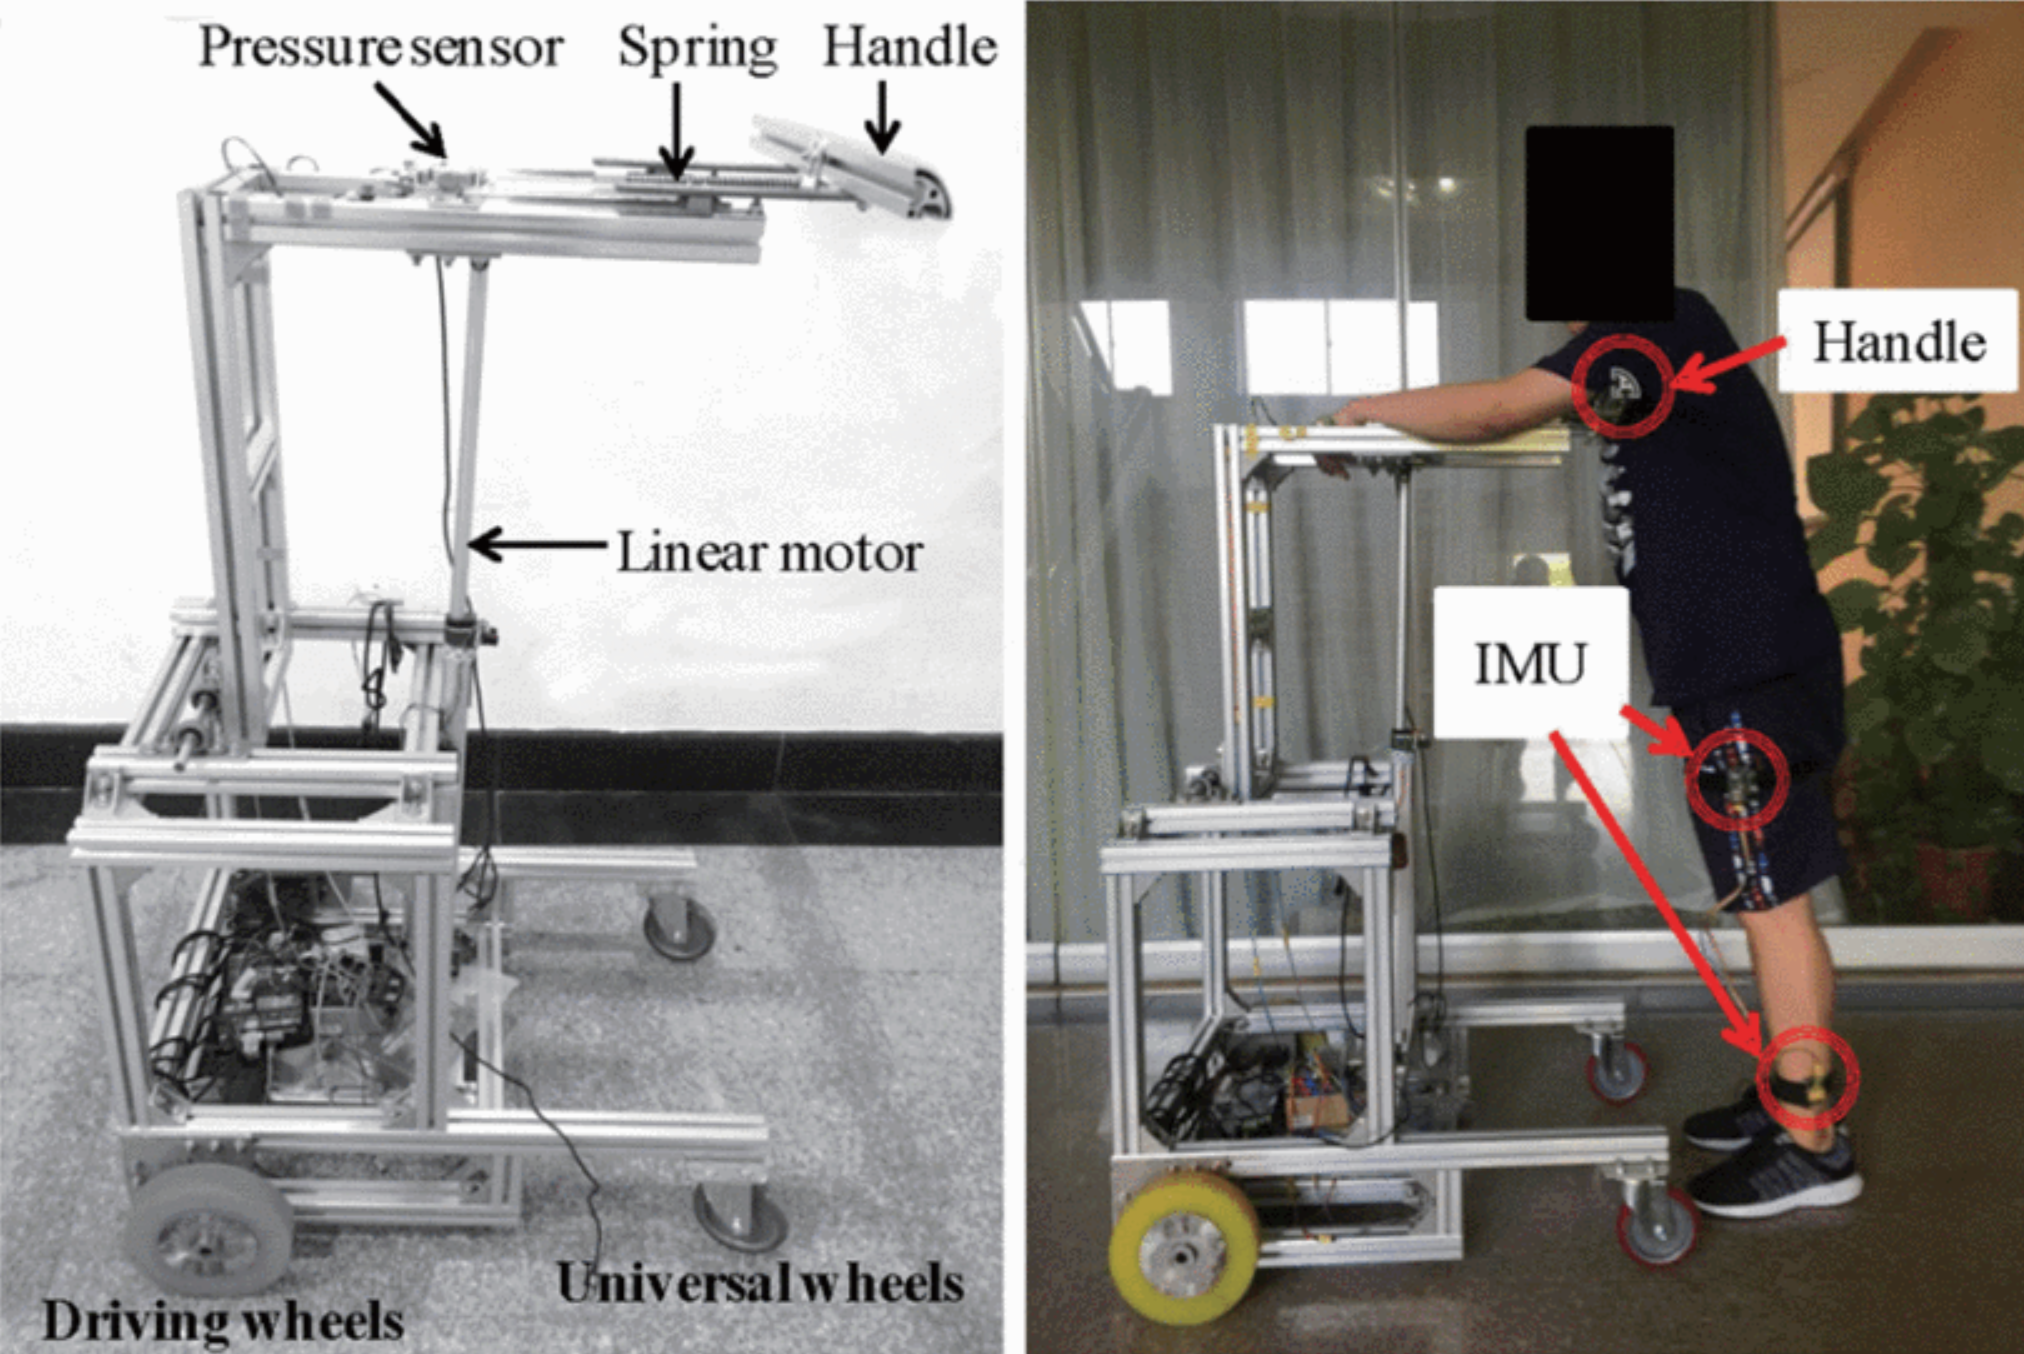
\includegraphics[width=\textwidth]{TESIS/imagenes/chap02/AplWalkerRobotic2.png}
\caption{ Andador robótico multifunción guiado por sensores de medición inercial y un modulo de transmisión de fuerza. \cite{walker8688067}}
\label{fig:robotic_walker}
\end{figure}

Un modulo de interfaz de usuario supervisa la progresión lineal en un grado de libertad utilizando sensores de medición. En base al principio bípedo, calcula el ángulo dinámico necesario para reflejar el movimiento cinemático, y así determinar las señales de control que serán enviadas a los controladores del motor. Finalmente, las señales recibidas son colocadas en un ciclo de retroalimentación que determinan los comandos del motor para controlar el andador robótico multifunción \cite{Modise2016}.

\section{Revisión Sistemática Basada en Evidencias} \label{fundamentos:RSBE}

Esta sección aborda el paradigma basado en evidencias, actualmente adoptado en muchas ciencias prácticas (i.e. medicina, educación, política social e ingeniaría). Las \gls{SLR} son un aspecto esencial del paradigma basado en evidencias, y tienen como objetivo sintetizar los estudios de investigación asociados a una pregunta de investigación específica, de forma rigurosa, auditable y justa. 

La presentación en cada subsección, describe el beneficio y el potencial de las revisiones sistemáticas de la literatura, razón por la cual será la metodología de investigación adoptada durante el proyecto PARKIBIP. Asimismo, procura especificar el flujo de actividades estándar a realizar en una SLR.

\subsection{Paradigma basado en evidencias}

Para lograr un mayor entendimiento se considera apropiado iniciar por el significado de \gls{evidencia} en un marco científico y tecnológico, ya que será aplicado a practicas de ingeniería de software en la realización de PARKIBIP.

En general, la evidencia se asocia al conocimiento. Normalmente se espera que el conocimiento se derive de la evidencia a través de algún proceso de interpretación (i.e. un modelo matemático o estadístico), y no basado en ilusiones. Por ejemplo, una ilustración menos científica ocurre cuando un jurado, en un juicio penal, tiene que considerar la evidencia de un conjunto de testigos para obtener un conocimiento razonable sobre lo sucedido. Asimismo, analizar dicho proceso por el cual se interpreta el primero para agregar o inferir el segundo es de suma importancia. Se detectan dos parámetros esenciales para producir evidencia solida a partir de un proceso de revisión objetiva: 

\begin{itemize}
    \item Selección objetiva e imparcial de estudios relevantes 
    \item Síntesis sistematizada de los resultados de los estudios previamente seleccionados
\end{itemize}

En resumen, la practica basada en evidencias (EBP, por sus siglas en ingles) busca utilizar un enfoque objetivo, riguroso y planificado para seleccionar estudios relevantes y realizar una sıntesis de los resultados de esos estudios \cite{Kitchenham2006}. La rigurosidad metodológica hace que los resultados sean mas confiables, ya que es posible estudiar el procedimiento llevado a cabo para su obtención ası como también reproducirlo.

La ingeniería de software basada en evidencias realiza un fuerte énfasis en el rigor metodológico involucrando los siguientes cinco pasos \cite{Kitchenham2004, Pizard}:

\begin{enumerate}
    \item Convertir un problema relevante o una necesidad de información en una pregunta que pueda ser respondida.
    \item Buscar en la literatura la mejor evidencia para responder a esa pregunta.
    \item Evaluar de forma crıtica la validez, el impacto y la aplicación de la evidencia.
    \item Integrar la evidencia evaluada con la experiencia practica y los valores y circunstancias de los interesados.
    \item Evaluar la efectividad y la eficiencia de este proceso para buscar maneras de mejorarlo.
\end{enumerate}

Los primeros tres pasos son esencialmente el papel de la revisión sistemática de literatura, mientras que el cuarto, es el de la traducción del conocimiento. El quinto es garantizar que los procedimientos de investigación estén sujetos a un análisis constante.

Para brindar una definición concisa a la técnica mencionada, es necesario clasificar las investigaciones en estudios:

\begin{itemize}
    \item Primarios: métodos utilizados para realizar estudios con el objetivo de obtener evidencia empírica sobre un tema de interés (i.e. encuestas, experimentos, estudios de caso, investigación y acción - del ingles, action research-).
    \item Secundarios: métodos que permiten recopilar de manera sistemática y rigurosa los estudios primarios relacionados con una pregunta de investigación específica, con el objetivo de sintetizar la evidencia disponible para responder a dicha pregunta (i.e.  revisión sistemática de literatura).
\end{itemize}

De esta manera, una revisión sistemática de literatura o SLR es un estudio secundario generado a partir de estudios primarios, y se define como un método para identificar, evaluar e interpretar todas las investigaciones pertinentes a una determinada pregunta de investigación, área, temática o fenómeno de interés. Es la principal herramienta del paradigma basado en evidencias, siendo sistemáticas -porque se conducen siguiendo un conjunto de procedimientos bien delineados y reproducibles-, además tratan de evitar sesgos, son rigurosas y abiertas.

La ilustración Fig. \ref{fig:context_srl} permite resumir mediante un esquema macro el flujo de información entrante y saliente relativo a una SLR; así como también el impacto futuro en políticas, estándares y practicas. 

\begin{figure}[H]
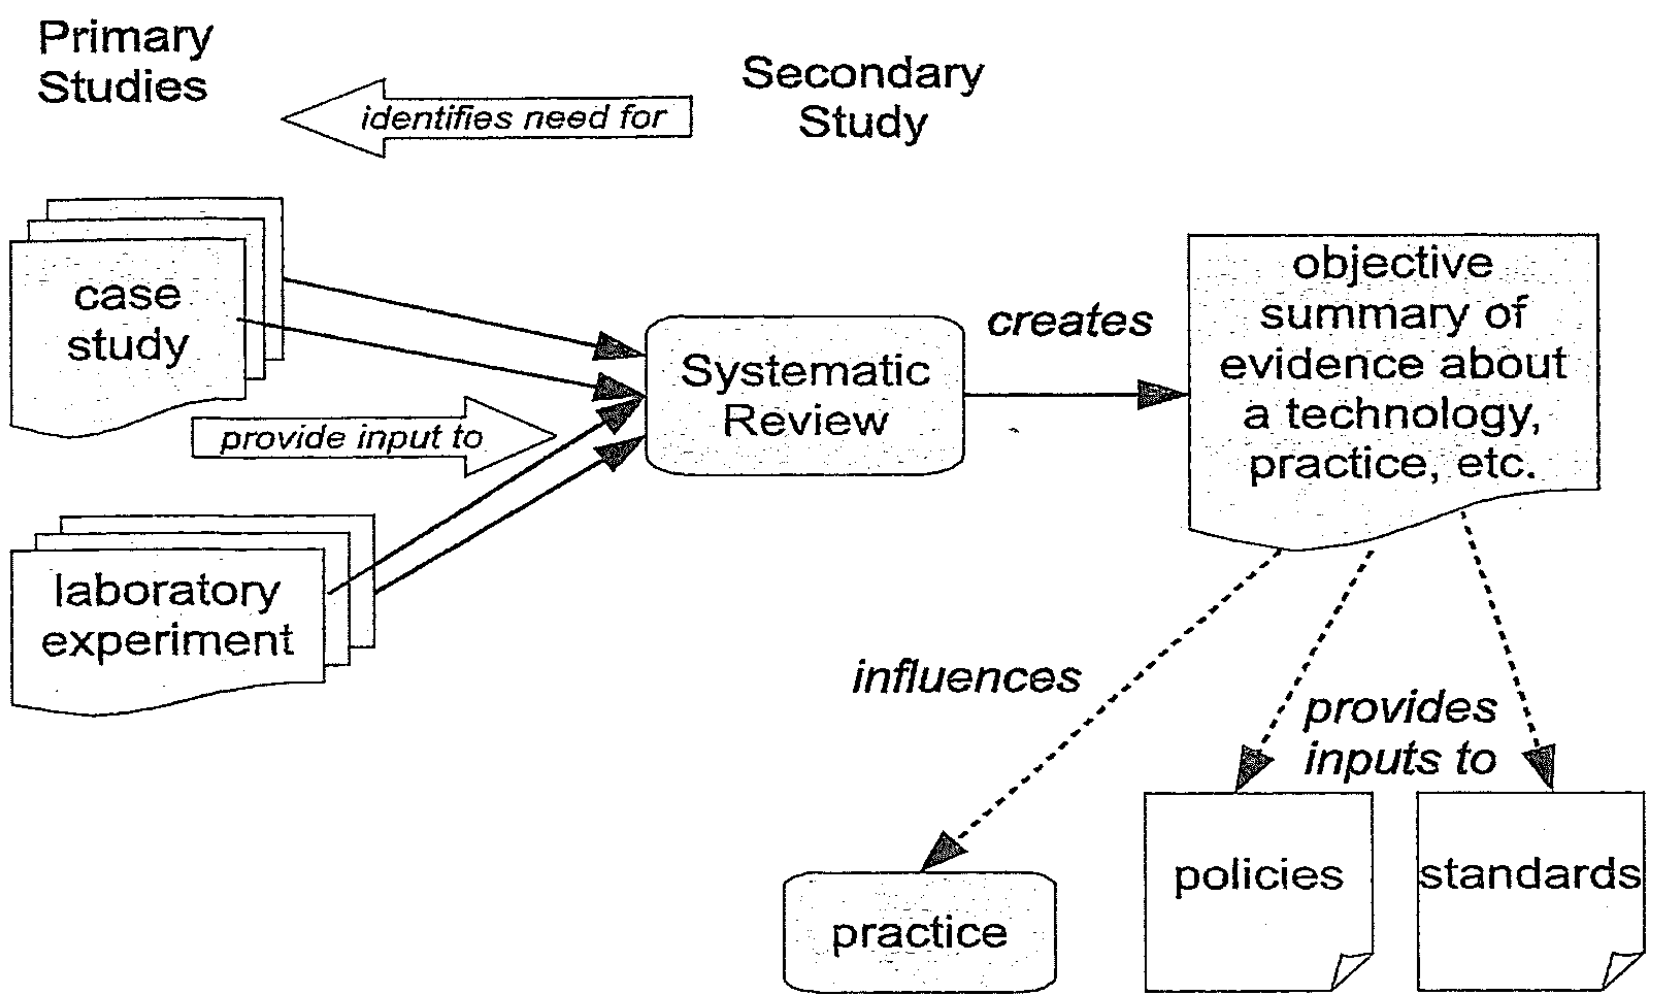
\includegraphics[width=\textwidth]{TESIS/imagenes/chap02/Contexto_RSL.PNG}
\caption{ Contexto de una revisión sistemática de literatura \cite{Kitchenham2006}.}
\label{fig:context_srl}
\end{figure}

\subsection{Revisión sistemática de literatura}

En general, los investigadores ejecutan las revisiones para resumir la evidencia científica existente sobre algún fenómeno particular, de manera exhaustiva e imparcial. Según una encuesta reciente, los principales factores de motivación en la ingeniería de software son:

\begin{itemize}
    \item Reunir conocimiento respecto a un campo o estudio en particular.
    \item Identificar recomendaciones para investigaciones futuras.
    \item Establecer el contexto de un tema o problema de estudio.
    \item Identificar las principales metodologías y técnicas de investigación usadas en un campo de investigación particular.
\end{itemize}

\noindent Realizar una revisión sistemática es un proceso extremadamente lento, que requiere suma atención en los detalles. Siempre es bueno comenzar por establecer la necesidad (i.e. ya existe otra que aborde el mismo tema) y por ende la motivación de ejecutar una revisión, para luego evaluar su factibilidad. 

Asimismo, especificar los aspectos técnicos del proceso de revisión (planeamiento) es un factor fundamental para lograr resultados satisfactorios. Esto es, desarrollar un protocolo de revisión que permita realizar y documentar las estrategias y toma de decisiones de diseño del estudio. Su definición de antemano puede ayudar a reducir la probabilidad de sesgo, limitando la influencia de las expectativas del investigador (i.e. la selección de estudios primarios o la síntesis de los resultados). A modo de ejemplo se propone la Tabla \ref{tab_protocolcomponents},que sugiere los componentes a incluir en un protocolo de revisión.
\begin{table}[H]
    \begin{center}
     \caption{\label{tab_protocolcomponents} Componentes de un protocolo de revisión}
        \begin{tabular}{ |p{12cm}| } 
        \hline
        Antecedentes y justificación de la revisión. \\
        \hline
        Preguntas de investigación.\\
        \hline
        Estrategia de búsqueda para estudios primarios. Debe incluir los términos de búsqueda y recursos donde se realizar´a la búsqueda. Los recursos incluyen librerıas digitales, revistas especıficas, y actas de congresos.\\
        \hline
        Criterios de selección de estudios. Usados para determinar cuales estudios son incluidos o excluidos de la revisión sistemática.\\
        \hline
        Procedimientos de selección de estudios. El protocolo debe describir como se aplicar´a el criterio de selección, por ejemplo, cuantos asesores evaluaran cada estudio primario, y como se resolverán los desacuerdos entre los evaluadores.\\
        \hline
        Procedimientos y listas de verificación para evaluar la calidad.\\
        \hline
        Estrategia de extracción de datos.\\
        \hline
        Método o técnica de sıntesis de los datos.\\
        \hline
        Limitaciones.\\
        \hline
        Estrategia de difusión.\\
        \hline
        Calendario del proyecto de revisión.\\
        \hline
        \end{tabular}
    \end{center}
\end{table}

\noindent Dentro de la fase de planeamiento, otro ítem sumamente determinante, es establecer las preguntas de investigación que guiarán e incidirán en todo el estudio (i.e. que estudios primarios incluir o excluir, decidir que datos deben extraerse y cómo sintetizar los datos para contestar las preguntas). Una pregunta es adecuada cuando \cite{Kitchenham2004}:

\begin{itemize}
    \item Es significativa e importante tanto para investigadores como para profesionales.
    \item Dará lugar a cambios o incrementará la confianza en las practicas actuales de la ingenierıa de software.
    \item Identificará las discrepancias entre las creencias comúnmente aceptadas versus la realidad.
\end{itemize}

Posterior a la etapa de diseño o planeamiento, inicia la fase de ejecución de la revisión sistemática. Si bien no será objeto de aplicación en el proyecto PARKIBIP, y por lo tanto no será analizada con detenimiento, es importante mencionar la última etapa de Documentación y publicación del estudio. El esquema en la figura Fig. \ref{fig:review_phases} expone un patrón organizado y sistemático a seguir en la realización de una SLR. De igual manera, incluye la clasificación en fases y el protocolo de revisión mencionados anteriormente.

\begin{figure}[h!]
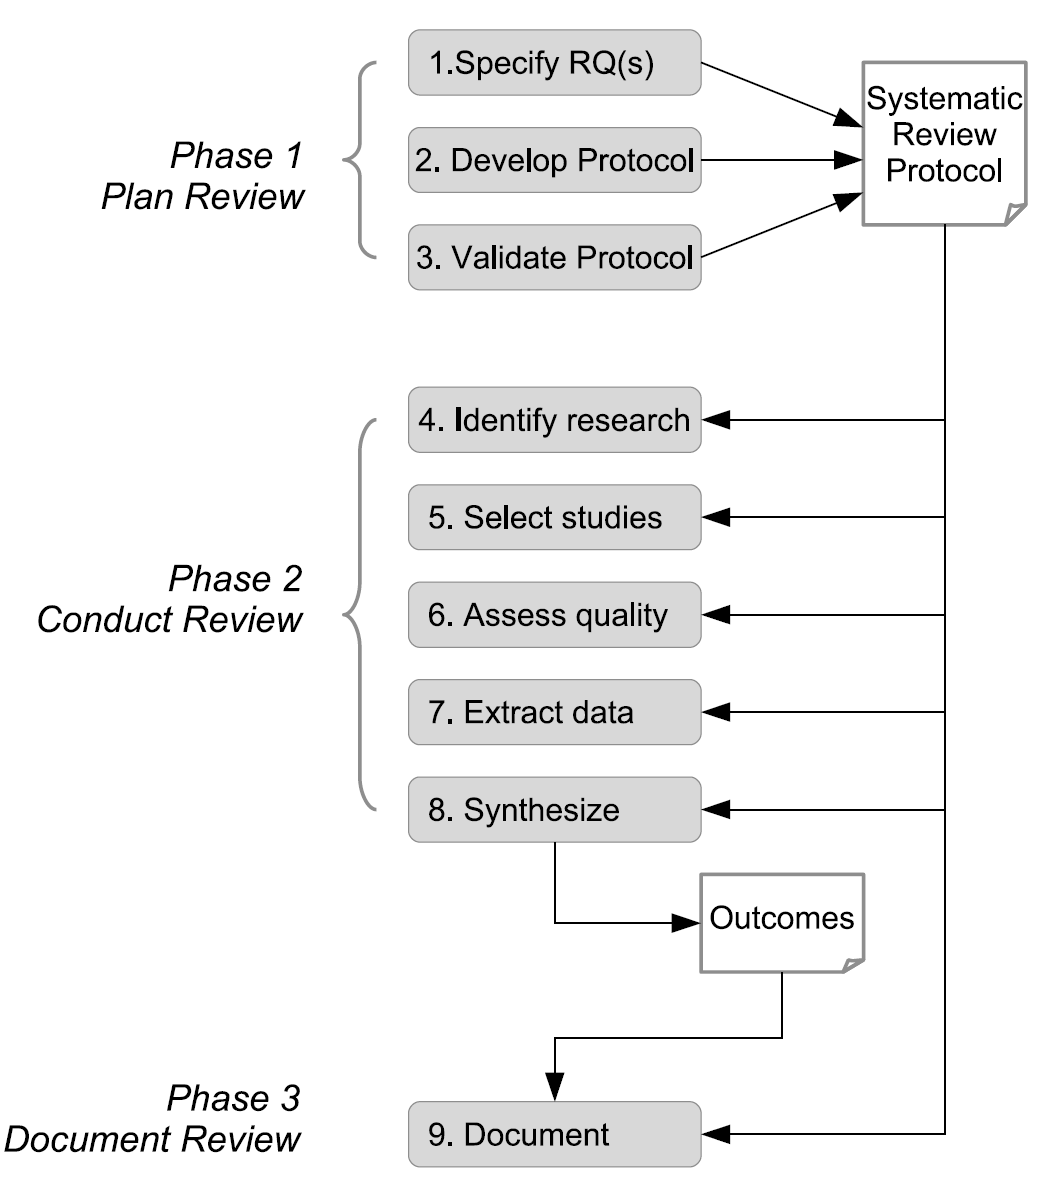
\includegraphics[width=\textwidth]{TESIS/imagenes/chap02/review_phases.PNG}
\caption{Flujo de actividades en el proceso de una SLR. \cite{Kitchenham2006}}\label{fig:review_phases}
\end{figure}

En resumen, una SLR tiene ciertas etapas discretas contempladas en tres fases principales, cada una con sus actividades particulares:
\begin{enumerate}
    \item Planificar la Revisión 
    \begin{itemize}
        \item Especificar las preguntas de investigación.
        \item Desarrollar el protocolo de revisión.
        \item Evaluar el protocolo de revisión (recomendada).
    \end{itemize}
    \item Realizar la Revisión
    \begin{itemize}
        \item Identificar la investigación.
        \item Seleccionar los estudios primarios.
        \item Evaluar la calidad de los estudios.
        \item Extraer datos y monitorear.
        \item Sintetizar los datos.
    \end{itemize}
    \item Informar la Revisión
    \begin{itemize}
        \item Especificar los mecanismos de difusión.
        \item Formatear el informe principal.
        \item Evaluar el informe (recomendada).
    \end{itemize}
\end{enumerate}

Es relevante notar, que la lista de fases de una revisión sistemática es una guía sugerida y bien estructurada. Además, no es estrictamente secuencial y algunas pueden repetirse mas de una vez, involucrar iteraciones o de ser necesario volver a ejecutar etapas. En otras palabras, el proceso podrá tener variaciones al caso típico y dependerá exclusivamente del contexto de aplicación, las necesidades y las limitaciones del proyecto, así como también las decisiones de los revisores.

A continuación, se hará una breve introducción a las principales actividades de la fase ``Realizar una revisión sistemática''. Comprender el propósito y aplicación de cada sub-etapa, será sustancial para acompañar con éxito el desarrollo de la metodología en el proyecto PARKIBIP -Cap. \nameref{chap_RSBE}-. 

\begin{enumerate}[label=(\roman*)] 
\item Identificar la investigación. En esta etapa se establece y utiliza una estrategia de búsqueda para obtener una lista de todas las publicaciones relevantes para las preguntas de investigación. La estrategia de búsqueda puede ser automatizada mediante librerías digitales, búsquedas manuales, o mediante contactos con los investigadores; pero tiene que estar definida en el protocolo de la revisión y debe ser reportada luego de forma transparente y replicable. Una alternativa de búsqueda -a veces utilizada como complemento-, es el uso de las referencias en la búsqueda de nuevos estudios. Iniciando desde un estudio primario de interés, para luego emplear sus referencias para encontrar nuevos estudios relevantes (\gls{backward_snowballing}) o se buscan cuales estudios lo ubican en sus referencias (\gls{forward_snowballing}). En caso de utilizar una búsqueda automatizada, se debe incluir una descripción de la cadena de búsqueda y los recursos utilizados.
  \item Seleccionar los estudios primarios. En este paso se establecen los criterios de selección de artículos primarios, que determinarán aquellas publicaciones que serán incluidas -Crit. Inclusión, definen qué estudios se deben incluir como relevantes- o excluidas -Crit. Exclusión, se aplican sobre los estudios seleccionados o sobre la lista inicial para remover estudios irrelevantes- de la revisión. Los criterios de selección pretenden identificar los estudios primarios que proporcionan evidencia directa acerca de las preguntas de investigación. Según el procedimiento estipulado, el procedimiento de selección de artículos puede basarse en la lectura rápida de la combinación titulo, resumen, palabras claves de las publicaciones primarias -en general, se tienen muchos artículos, y es imposible leerlos por completo-.
  \item Evaluación de calidad. Evaluar la calidad de un articulo es una actividad desafiante, y conlleva a establecer qué parámetros de calidad serán evaluados y el procedimiento para su aplicación. En general es adecuado definir un lista de chequeos (del ingles, checklist) en base a preguntas concisas y proceder a aplicarlos de tal forma que asegure la mejor calidad de la evaluación. La calidad se refiere a la medida en que el estudio minimiza el sesgo y maximiza tanto la validez interna como la externa.
  \item Extracción de datos. El objetivo de esta etapa es el diseño de formularios de extracción de datos para que los investigadores puedan registrar adecuadamente la información que se obtiene de los estudios primarios. El formulario deberıa incluir información asociada a la extracción, información general del estudio,(i.e. identificador del estudio, titulo y detalles de publicación), preguntas que habiliten a responder las preguntas de investigación, preguntas para evaluar la calidad de los estudios y resumen de los datos.
  \item Síntesis de datos. La síntesis es el proceso en el cual se recolectan, integran y resumen los hallazgos incluidos en los estudios primarios. Sin importar el tipo de síntesis -descriptiva (o narrativa) y cuantitativa-, se debería comenzar con la creación de un resumen de los estudios incluidos, presentando intervenciones, numero y característica de los participantes, resultados, entre otros. Una alternativa es realizar una síntesis temática y narrativa, en donde los datos se presentan tabulados, de tal forma que sean consistente con las preguntas de investigación. Es relevante notar, que el resultado de la síntesis es el disparador para las conclusiones finales.
\end{enumerate}

\section{Análisis de la marcha}

En los últimos años, el análisis de la marcha y la partición de sus fases ha sido un tema de investigación desafiante debido a su impacto en muchas aplicaciones relacionadas con tecnologías de la marcha. El paso o la marcha humana es un proceso complejo y cíclico que requiere la sinergia de los músculos del cuerpo, los huesos y el sistema nervioso \cite{SAUNDERS1953}, principalmente dirigido a mantener la posición vertical y mantener el equilibrio durante condiciones estáticas y dinámicas \cite{Ayyappa1997}. 

El análisis de la marcha o \gls{gait_analysis} instrumentado provee mediciones confiables y objetivas sobre los patrones de locomoción y su variabilidad. Estas mediciones, pueden contribuir a la investigación de patologías y definición de programas de rehabilitación. GA está emergiendo como una herramienta efectiva para detectar enfermedades neurodegenerativas o para monitorear su progresión \cite{Bertoli2018}. Específicamente, los parámetros de la marcha son indicadores útiles para discriminar enfermos de Parkinson así como para cuantificar la severidad de la enfermedad. Aprovechando los modelos cinemáticos, los sistemas pueden identificar ciertos patrones en las señales para detectar pasos y calcular parámetros; como la cadencia, la longitud de zancada, la velocidad de zancada, el rango de movimiento, los ángulos de las articulaciones, la velocidad máxima de oscilación, sentarse para pararse y pararse para sentarse, tiempos de transición, tiempo de giro, velocidad máxima de giro, etc. Estos parámetros han mostrado una correlación significativa con el diagnóstico de la enfermedad de Parkinson y la cuantificación de su severidad \cite{Akbari2017}.

\subsection{Identificación de fases de la marcha}

El ciclo de la marcha se define como el período de tiempo que transcurre desde el contacto inicial de un pie con el piso, hasta la próxima ocurrencia del mismo evento en el mismo pie. Existen muchos modelos de partición de dicho ciclo, con diferentes niveles de granularidad, que dependen de los objetivos clínicos: el modelo que incluye dos grandes fases de la marcha, es decir, apoyo y vuelo, es en general el más adoptado según la revisión sistemática de \cite{Taborri2016}; la cual recopila una gran variedad de estudios dentro del GA así como los distintos modelos empleados para distinguir el ciclo de la marcha en sus respectivas fases. La siguiente figura Fig. \ref{fig:gait-phases}, condensa los distintos hallazgos y nomenclaturas empleadas en la literatura respecto a las granularidades del ciclo de la marcha.

\begin{figure}[H]
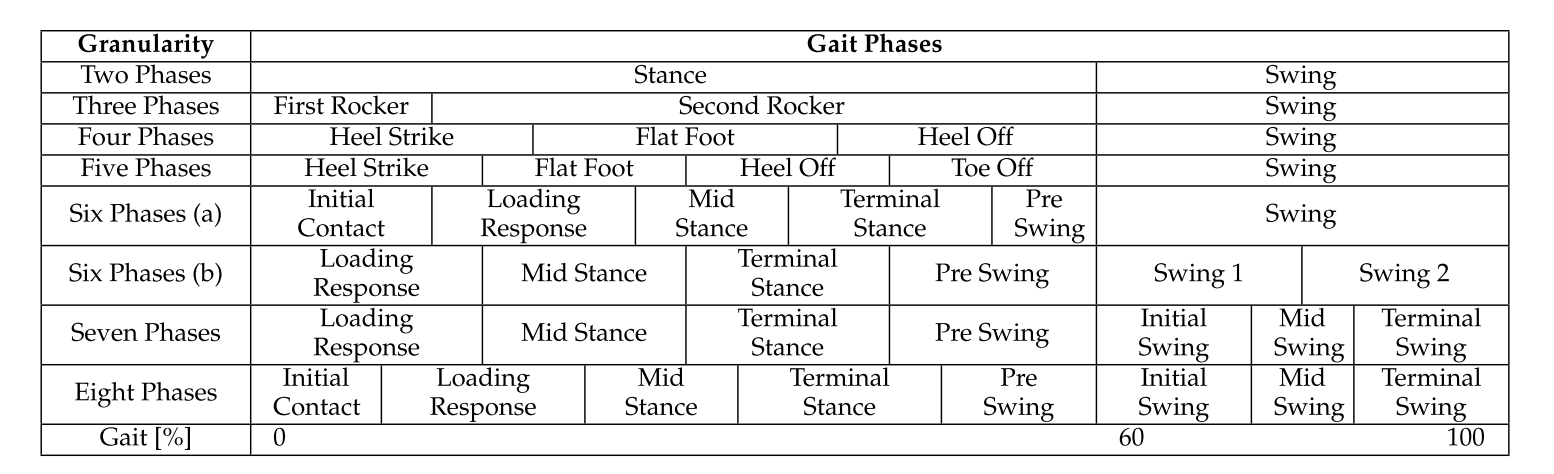
\includegraphics[width=\textwidth]{TESIS/imagenes/chap02/Gait-phases-classification.png}
\caption{ Nomenclatura para diferentes granuralidades del ciclo de marcha \cite{Taborri2016}.}
\label{fig:gait-phases}
\end{figure}

La correcta discriminación de las fases de la marcha es considerado un punto de partida para muchas aplicaciones, por ejemplo: (i) la evaluación del estado de recuperación de la marcha durante tratamientos de rehabilitación o luego de alguna intervención; (ii) la clasificación de las distintas actividades de la vida diaria o AVD; (iii) el control sinérgico de los dispositivos robóticos, para la recuperación de la movilidad de las extremidades inferiores; (iv) el entrenamiento atleta; y finalmente, (v) para distinguir una marcha normal de una patológica \cite{Taborri2016}.

\subsection{Sensores de medición para análisis de la marcha}

Una variedad de sensores pueden ser utilizados para alimentar algoritmos que identifican las distintas fases de la marcha, clasificados principalmente como vestibles o no vestibles - del ingles \gls{Wearables} y \gls{non_Wearables} respectivamente- . Dentro de los sensores vestibles, las plantillas de presión (en inglés ``footswitches'') son consideradas un estándar  \cite{Taborri2016}; sin embargo, para resolver algunas limitaciones inherentes en estos dispositivos, las unidades de medición inercial se han vuelto muy populares en la última década. Buenos resultados han sido alcanzados utilizando también sensores de ultrasonido, electro-miografías (EMG) y electro-neurografías (ENN). 

Los sensores no vestibles, como los sistemas optoelectrónicos o las plataformas de fuerza, se mantienen como los sistemas más precisos para analizar la marcha en ambientes interiores. A pesar de su utilidad, han tenido un uso muy limitado, especialmente en países en desarrollo, debido al alto costo que implica establecer un laboratorio especializado de marcha. La principal desventaja de este tipo de sistemas, es que no proveen una evaluación de los pacientes durante sus actividades cotidianas, extrapolando las conclusiones de un estudio de corto tiempo que no refleja las condiciones reales del paciente. Además, la evaluación puede requerir mucho tiempo y puede ser difícil de tolerar por los sujetos, principalmente si se trata de condiciones patológicas \cite{Kumar8372660}.

Resulta fundamental para el proyecto PARKIBIP identificar el tipo apropiado de sensor que se utilizará para nutrir los algoritmos, que luego detectarán las distintas fases de la marcha en tiempo real. Es inherente al objetivo del proyecto que el tipo de sensor debe ser del tipo vestible o wearable, ya que el sistema debe ser portable y utilizable en ambientes exteriores. Una revisión sistemática basada en evidencias del año 2016 \cite{Taborri2016} identifica, selecciona y categoriza las distintas metodologías utilizadas para la detección de fases de la marcha, analizando ventajas y desventajas de cada una de las soluciones. 

Los pedales (en inglés, ``footswitches'') son dispositivos que emplean sensores capaces de detectar el contacto del pie con el piso durante un ciclo de marcha. Se emplean principalmente para medir parámetros temporales en la marcha. Estos sensores, que van colocados en la parte inferior del pie, operan como interruptores y se encuentran conectados por cables a algún tipo de terminal. Al ser de bajo costo y proveer una precisión muy alta, son usualmente utilizados para complementar la medición de otro tipo de sistema. Sin embargo, presentan varias desventajas claves para PARKIBIP, como por ejemplo: (i) el número de fases detectables es limitado, dado que las sub fases en la etapa de vuelo del pie no pueden ser discriminadas; (ii) el lugar en el que son dispuestos los sensores, en los pacientes con marcha patológica, afecta la precisión y la confiabilidad de medición \cite{AMINIAN2002689}; por ultimo, (iii) la conexión cableada afecta la oportunidad del sistema de ser un instrumento para las actividades de la vida diaria de los sujetos afectados.

Las plantillas de presión o ``Foot Pressure Insoles'', presentan ventajas y desventajas similares a los pedales, ya que se basan en los mismos principios. Si bien existen plantillas que no requieren cableado, por ende no presentan dicha desventaja, éstas son de un costo elevado en comparación a los pedales u otras soluciones (p. ej. los sensores de aceleración, giroscopios o incluso las unidades de medición inercial). 

El acelerómetro es la solución más utilizada para el análisis del paso ambulatorio. Con el objetivo de reconocer las fases del paso de un individuo, la evidencia literaria existente describe diferentes combinaciones de éstos sensores, junto a los posibles lugares donde pueden ser ubicados. Los acelerómetros, entre otras unidades inerciales, son relativamente pequeños, de baja energía y larga autonomía, baratos, portables y altamente accesibles en la industria \cite{TongKaiyuGranat1999}. En comparación con las soluciones basadas en pedales o plantillas ya mencionadas, el análisis de la aceleración ha permitido a los investigadores distinguir ciertas fases de la marcha, como lo es la sub-fase de etapa de vuelo (o en ingles, fase de Swing). Sin embargo, el empleo de acelerómetros para identificar las fases de la marcha, implica ciertas complejidades que resultan críticas: (i) la necesidad de compensar la gravedad durante el cómputo de la aceleración, de la parte del cuerpo analizada; (ii) el error acumulado en la integral doble aplicada al conjunto de datos sensados, para el cálculo de la posición; y, (iii) el procedimiento de calibración que permite ubicar de forma correcta el sensor respecto a un estándar de referencia trazable, y así confiar en la validez de sus mediciones.

La velocidad angular -como una variable para la partición de las fases del paso-, dato extraído desde el dispositivo giroscopio, ha adquirido una gran popularidad en las últimas décadas y es preferida sobre otras variables inerciales. La velocidad angular no se encuentra afectada por la gravedad, como tampoco la curva de sus ondas por el toque del talón con el suelo (a.k.a. ``heel strike''). Además, no es necesario mantener un cuidado minucioso respecto a la posición en donde es ubicado el giroscopio dentro del segmento del cuerpo a medir. Aunque, una desventaja en su utilización es que, tal como la aceleración, la velocidad angular también se ve alterada por el error propagado, en caso de que se compute el ángulo del movimiento. 

\subsection{Unidad de Medición Inercial (IMU)}

La Unidad de Medición Inercial, también conocida como IMU (Inertial Measurement Unit, por sus siglas en inglés), combina varios de los sensores mencionados, como por ejemplo el acelerómetro y el giroscopio; algunos también incluyen magnetómetro, barómetro, sensores de luz y/o temperatura, entre otros. 

Por su parte, los dispositivos IMUs presentan una serie de ventajas que hace con que sea el tipo de dispositivo adecuado para el proyecto PARKIBIP. A continuación, se listan algunas de ellas \cite{ZAGO201844}:

\begin{itemize}
    \item La combinación de diferentes cantidades inerciales permite la evaluación de diferentes tipos de primer contacto con el piso, el cual representa un índice sumamente importante para analizar el estado de salud del sujeto, utilizando la estimación de la orientación del pie. 
    \item La fusión de los datos de velocidad angular y aceleración lineal permiten compensar el error acumulado. 
    \item Estos dispositivos permiten la evaluación en tiempo real de los parámetros espacio-temporales en entornos de la vida real, interiores y exteriores, superando así las limitaciones típicas de las mediciones de laboratorio.
    \item Los IMUs son más baratos y más prácticas que los sistemas de GA completos; solo se requiere una preparación relativamente rápida de los pacientes, ya que el sensor se coloca en el cuerpo por medio de un cinturón elástico.
    \item Los datos se pueden transferir fácilmente a través de Bluetooth al software dedicado.
\end{itemize}

Si bien el dispositivo tiene un gran potencial para el proyecto PARKIBIP, se deberán tener en cuenta ciertos factores que pueden afectar la señal de entrada y salida \cite{Anwary8246577}. Por ejemplo, durante la caminata, el movimiento de la ropa puede causar interferencias con la salida del acelerómetro. Puede haber vibración o ruido causado por el impulso si el sensor no es ajustado correctamente. Ajustar el sensor en un cinturón o cargarlo en el bolsillo también puede inducir interferencia de movimiento relativo. Para aumentar la confiabilidad y validez de la extracción automática de los parámetros para el análisis de la marcha, es fundamental elegir correctamente el lugar donde serán colocados los sensores y la forma en la que se coloquen. 